\documentclass[draft]{agujournal2018}
\usepackage{apacite}
\usepackage{url} %this package should fix any errors with URLs in refs.
%\usepackage{lineno}
%\linenumbers


%\drafttrue
\draftfalse
\journalname{JGR: Earth Surface}

%% you probably have to kill these custom commands later %% 
\newcommand\be{\begin{equation}} % shortcut to start eq envs 
\newcommand\ee{\end{equation}}   % shortcut to end eq envs
\newcommand\bra{\langle}
\newcommand\ket{\rangle}
\usepackage{amsmath,amssymb,amsfonts,amsthm}
\usepackage{comment}
\usepackage{wrapfig}
\usepackage{lipsum}
\usepackage{booktabs} % for wrapping text around tabulars in accord with
% https://tex.stackexchange.com/questions/49300/wrap-text-around-a-tabular
\usepackage{ragged2e}
\justifying

\begin{document}

\title{Joint stochastic theory of bedload transport and bed elevations: derivation of heavy-tailed resting times}
\authors{James K. Pierce\affil{1}\thanks{Vancouver, British Columbia, Canada}, and Marwan A. Hassan\affil{1}}
\affiliation{1}{Department of Geography, University of British Columbia}
\correspondingauthor{James K. Pierce}{kpierce@alumni.ubc.ca}

\begin{keypoints}
\item We model fluvial bedload activity and local bed elevation as a two-species stochastic birth-death process.
\item Computations show heavy-tailed power-law distributions of resting times for sediment undergoing burial, with universal tail parameters $\alpha\approx1.15$.
\item We discuss implications for bedload diffusion and suggest a new theoretical framework to approach the problem.

\end{keypoints}

\begin{abstract}
A consensus has formed that fluvial bedload resting times lie on heavy-tailed statistical distributions which may result from sediment burial.
However, due to observational difficulties, only a handful of experiments have resolved these distributions, and there have been few theoretical attempts to build understanding, leaving their generating mechanism and specific characteristics uncertain.
With reference to these issues, we present a new theory describing bedload transport and bed elevation changes as a joint stochastic process, deriving resting time distributions for sediment undergoing burial from the joint dynamics.
Our theory predicts heavy-tailed power-law distributions of resting times with universal tail behavior completely characterized by the mean erosion rate and its scaling with bed elevation changes.
\end{abstract} 

\section{Introduction}

% bulk transport vs. individual grains & relevance of research
The majority of classic studies into fluvial sediment transport have attempted to relate the bulk downstream flux of bedload to characteristics of the hydraulic forcing \citep[e.g.][]{Yalin1972}, yet the relevance of this approach to environmental problems is limited, as many contemporary issues require knowledge of differences between motions of individual grains, and not just average characteristics.
For example, the export of contaminants from channels \citep[e.g.][]{Malmon2005} and the morphological response of channels to ecological restoration efforts \citep[e.g.][]{Gaeuman2017} or changes in hydrology or sediment supply \citep[e.g.][]{Hassan2017} are not described by bulk fluxes, highlighting individual sediment motions as an important topic for geophysics research.

A significant complication is that individual grains transport within a noisy environment, which noise sources ranging across spatial and temporal scales from fluid turbulence \citep{Celik2014} and the variable arrangement of bed surface grains \citep{Gordon1972}, to channel morphology changes \citep{Hassan2017} and unsteady flows \citep{Phillips2013}.
As a result, the transport characteristics of individual grains are not deterministic \citep[e.g.][]{Einstein1937}, even in the most controlled laboratory experiments \citep[e.g.][]{Charru2004, Bohm2004, Fathel2015, Heyman2016}.

This led researchers to create probabilistic theories of individual motions based on random walk concepts, whereby bedload motions are approximated as alternating sequences of steps and rests, with step lengths and resting times treated as random variables associated with statistical distributions \citep{Einstein1937, Yano1969, Nakagawa1976, Hassan1991, Bradley2012}.
In these theories, differences between the random motions of one grain and the next imply bedload diffusion, or a spreading apart of grains as they transport.
The diffusion characteristics predicted by these models critically differ depending on whether the step length and resting time distributions have light or heavy tails \citep[e.g.][]{Bradley2017}.

Heavy-tailed distributions have exceedance functions $P(X>x) \sim x^{-\alpha}$ with tail parameters $\alpha < 2$, meaning large values of $x$ are relatively common, while light-tailed distributions have $\alpha \geq 2$, meaning large values of $x$ are relatively rare.
If both resting time and step distance distributions have light tails, the diffusion is said to be normal or Fickian, with a variance of particle positions $\sigma_x^2$
scaling with time $t$ as $\sigma_x^2 \propto t$.
However, if either distribution has a heavy-tail, the diffusion is called anomalous, with a variance of particle position scaling as $\sigma_x^2 \propto t^\gamma$, where $\gamma\neq 1$.
In this expression, $\gamma <1$ is called sub-diffusion and $\gamma > 1$ is super-diffusion.
In strongly asymmetric random walks such as bedload transport, heavy-tailed step lengths imply super-diffusion, while heavy-tailed resting times imply either super or sub-diffusion, depending on $\alpha$ \citep{Weeks1996, Weeks1998}.

Tracer experiments in gravel bed rivers show anomalous bedload diffusion \citep{Phillips2013, Bradley2017}, light-tailed step lengths \citep{Bradley2012, Hassan2013}, and heavy-tailed resting times \citep{Voepel2013, Olinde2015, Pretzlav2016, Bradley2017}, forming a coherent experimental picture of super-diffusive bedload transport, at least at long observation timescales \citep[e.g.][]{Nikora2002, Martin2012}.
However, field studies have not resolved the mechanism generating these heavy-tailed resting times \citep[e.g.][]{Bradley2017}, and empirical distributions display clear differences in their form and characteristics, showing different tail parameters \citep[e.g.][]{Olinde2015} and sometimes truncation \citep[e.g.][]{Bradley2017} or tempering to light tails at large resting times \citep[e.g.][]{Voepel2013}.
The mechanism generating heavy tails and these differences deserve attention.

A predominant hypothesis is that heavy-tailed resting times and anomalous diffusion originate from sediment burial \citep{Voepel2013,Martin2014,Wu2019}.
Conceptually, when grains rest on the bed surface, material transported from upstream can deposit on top of them, preventing entrainment until it's removed, driving up resting times and imparting a heavy tail to the distribution.
\citet{Martin2014} have provided the only direct support for this hypothesis.
They traced grains in a narrow flume with clear sidewalls, directly resolving burial as the generator of heavy-tailed resting times, and they described their results with a theoretical model, formally similar to an earlier effort by \citet{Voepel2013}.

The models of \citet{Voepel2013} and \citet{Martin2014} treat bed elevations as a random walk and interpret resting times as return periods from above in the bed elevation time-series \citep[e.g.][]{Redner2007}.
Both models are successful in describing different experimental resting time distributions.
However, the assumptions and results of these models are inconsistent with one another, and their treatment of bed elevations as a process independent of sediment transport is questionable, since erosion and deposition are the source of bed elevation changes \citep[e.g.][]{Wong2007}, suggesting further study is necessary.

In this work, we approach the problem from a different angle, making an extension of the stochastic bedload transport theory of \citet{Ancey2008} to link bed elevation changes to the erosion and deposition events of individual grains, and we derive resting times as a consequence of this theory.
The key assumptions of our model are: (1) bedload erosion and deposition can be characterized by probabilities per unit time, or rates \citep[e.g.][]{Einstein1950, Ancey2008}; and (2) these rates are contingent on the local bed elevation, encoding the property that erosion of sediment is emphasized from regions of exposure, while deposition is emphasized in regions of shelter \citep[e.g.][]{Sawai1987, Wong2007}.
Our theory generates heavy-tailed distributions with no tempering and a universal tail parameter $\alpha \approx 1.1$ for a particular non-dimensionalization of the resting time, showing close correspondence to the results of \citet{Martin2014} and suggesting a correction to some imperfections in their results.
We conclude the paper by framing our work in relation to earlier ideas and discussing the implications of this work on questions of individual bedload motions and anomalous diffusion.

\section{Stochastic theory}
\label{sec:theory}

% describe the set up 
We define a volume of downstream length $L$ which contains some number $n$ of moving particles in the water flow and some number $m$ of stationary particles composing the bed at some time $t$.
For simplicity, we consider all particles as approximately spherical with the same diameter $2a$, so their mobility and packing characteristics are similar.
Following \citet{Ancey2008}, we prescribe four events which can occur at any instant to modify the populations $n$ and $m$, and we characterize these events using probabilities per unit time, or rates.
These are: (1) migration of a moving particle into the volume from upstream ($n \rightarrow n+1$); (2) the entrainment of a stationary particle into motion within the volume ($m\rightarrow m-1$ and $n\rightarrow n+1$); (3) the deposition of a moving particle to rest within the volume ($m\rightarrow m+1$ and $n\rightarrow n-1$); and (4) the migration of a moving particle out of the volume to downstream ($n\rightarrow n-1$).
As the events occur at random intervals, they set up a joint stochastic evolution of the populations $n$ and $m$ characterized by a joint probability mass function (pmf) $P(n,m,t)$ having marginal pmfs $P(n,t) = \sum_m P(n,m,t)$ and $P(m,t) = \sum_n P(n,m,t)$ for the number of particles in motion and rest in the volume at $t$.
These concepts are depicted in figure \ref{fig:concept}.
\begin{figure}
  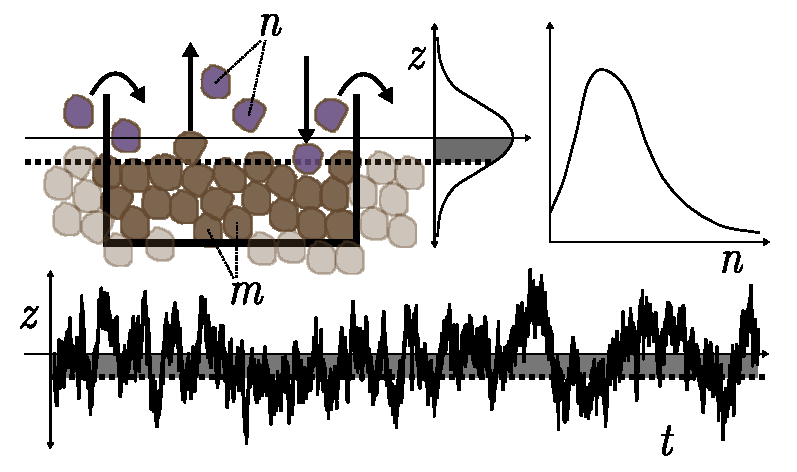
\includegraphics[width=\linewidth,keepaspectratio]{./figures/definition-combo.pdf}
  \vspace{-1.0cm}
  \caption{Definition sketch of a control volume containing $n$ moving grains and $m$ resting grains. Migration, entrainment, and deposition processes are represented by curved arrows, and the bed elevation at some instant is depicted by dotted line. The bed is presented in a degraded state, where $m<m_0$. The distributions of $n$ and $m$ are indicated in the upper right panel, while the bottom panel is a time-series of bed elevations (\ref{eq:ele}).}
  \label{fig:concept}
\vspace{-0.75cm}
\end{figure}

The populations $n$ and $m$ provide the bulk bedload flux $q_s$ and the local bed elevation $z$.
The mean bedload transport rate is given by $q_s \propto u_s \bra n \ket$, where $u_s$ is the characteristic velocity of moving bedload and $\bra n \ket = 
\sum_{n,m}nP(n,m) $ is the mean number of grains in motion \citep[e.g.][]{Charru2004, Ancey2008, Furbish2012a}.
The bed elevation is related to $m$ though the packing geometry of the bed.
To derive this, we prescribe a mean number of grains at rest $m_0$ and introduce a packing fraction $\phi$ of grains in the bed.
Then considering a two-dimensional bed \citep[e.g.][]{Einstein1950, Paintal1971}, the deviation from the mean bed elevation is
\be z(m) = \frac{\pi a^2}{\phi L}(m-m_0) = z_1(m-m_0). \label{eq:ele}\ee
The constant $z_1 = \pi a^2/(\phi L)$ is an important scale of the problem. 
$z_1$ is the magnitude of bed elevation change (in an average sense across the control volume) associated with the addition or removal of a single grain.
We write the rates of the four possible transitions as \citep[e.g.][]{Ancey2008}:
\begin{align}
 &R_{MI}(n+1,m|n,m) = \nu & \text{migration in}, \label{eq:rate1}\\
 &R_E(n+1,m-1|n,m) =\lambda(m) + \mu(m) n  & \text{entrainment},  \label{eq:rate2}\\
 &R_D(n-1,m+1|n,m) =\sigma(m) n & \text{deposition},\label{eq:rate3}\\
 &R_{MO}(n-1,m|n,m) =\gamma n & \text{migration out\label{eq:rate4}}.
\end{align}
These rates are independent of the past history of the populations and depend only on the current populations $(n,m)$. 
As a result, the system is Markovian \citep[e.g.][]{Cox1965, VanKampen1992}, meaning time intervals between subsequent transitions are exponentially distributed \citep[e.g.][]{Gillespie2007}.

In (\ref{eq:rate1}-\ref{eq:rate4}), $\nu$ and $\gamma$ are constants characterizing migration rates of individual grains into and out of the volume. 
They lack any dependence on the populations $n$ and $m$.
In contrast, $\lambda(m)$, $\mu(m)$, and $\sigma(m)$, characterizing the entrainment, collective entrainment \citep[e.g.][]{Ancey2008, Heyman2013, Heyman2014}, and deposition rates of individual grains are considered to depend on $m$.
As is well-known, bed elevation changes modify the likelihood of entrainment and deposition in a negative feedback \citep{Sawai1987, Wong2007}; that is, aggradation increases the likelihood of entrainment, while degradation increases the likelihood of deposition.
\citet{Wong2007} concluded that bed elevation changes induce an exponential variation in entrainment and deposition probabilities, while \citet{Sawai1987} concluded that the variation is linear.
For simplicity, we incorporate the scaling of \citet{Sawai1987} and note its equivalence to the \citet{Wong2007} scaling when bed elevation changes are small.
Because experimental distributions of bed elevations are usually symmetrical, \citep{Wong2007, Singh2009, Martin2014}, we expect the erosion and deposition feedbacks to be anti-symmetrical.
That is, as bed elevation changes drive up (down) erosion rates, so they drive down (up) deposition rates to the same degree.


% set up the m dependence of the rates
Summarizing these ideas, the entrainment and deposition rates can be written $\chi(m) = \chi_0(1\pm z_1 z(m)/(2l)^2)$, where $\chi = \lambda, \mu, \sigma$, and the entrainment parameters take the plus sign, while deposition takes the minus, and we have introduced a length scale $l$.
As we'll see, the variance of bed elevation turns out to be given by $\text{var}(z) = (l z_1)^2$. Accordingly, $l$ characterizes the range of bed elevation variations, which could be interpreted as the active layer depth \citep[e.g.][]{Church2017}.
Another perspective is that $l$ is the distance of bed elevation change at which the entrainment and deposition rates are significantly affected.
With these substitutions, the local bed elevation-dependent entrainment and deposition rates (\ref{eq:rate2}-\ref{eq:rate3}) can be written:
\begin{align}
R_E(n+1,m-1|n,m)&=[\lambda_0 + \mu_0 n]\Big[1 + \frac{z_1z(m)}{(2l)^2}\Big], && &\text{entrainment}, \label{eq:rate5}\\
R_D(n-1,m+1|n,m)&=\sigma_0 \Big[1-\frac{z_1z(m)}{(2l)^2}\Big]n, && &\text{deposition}. \label{eq:rate6}
\end{align}
At $z(m)=0$, the rates reduce to those of the \citet{Ancey2008} theory.
Away from this elevation, entrainment and deposition are alternatively suppressed and accentuated depending on the sign of $z(m)$.


In terms of the transition rates (\ref{eq:rate1}-\ref{eq:rate6}), we can obtain the Master equation for the probability flow using the forward Kolmogorov equation $\partial P(n,m;t)/\partial t = 
\sum_{n',m'} R(n,m)P(n',m';t)$ \citep[e.g.][]{Cox1965, Gillespie1992, Ancey2008} as 
\begin{multline}
 \frac{\partial P}{\partial t}(n,m;t) =  
\nu P(n-1,m;t) + 
\{\lambda(m+1) + [n-1]\mu(m+1)\}P(n-1,m+1;t)\\ + 
[n+1]\sigma(m-1)P(n+1,m-1;t) + 
[n+1]\gamma P(n+1,m;t) \\- 
\{ \nu + \lambda(m) + n\mu(m) + n\sigma(m) + n \gamma \}P(n,m;t).
 \label{eq:master}
\end{multline}
The joint probability distribution $P(n,m;t)$ solving this equation will fully characterize the statistics of $n$ and $m$.
We anticipate that solutions will adjust from the initial conditions to a steady-state distribution $P_s(n,m)$, independent of time, if the constant factors in the transition rates are representative of equilibrium bedload transport conditions.
This Master equation describes a two-species stochastic birth-death model \citep[e.g.][]{Cox1965} of a type well-known in the population ecology literature \citep[e.g.][]{Pielou1977, Swift2002}.
In our context, the two species are the moving and stationary grains in the volume.

\section{Numerical simulations}

Unfortunately, (\ref{eq:master}) does not appear to admit an analytical solution (but see \citet{Swift2002} for a standard method which fails in this case).
The difficulty stems from the product terms between $n$ and $m$.
In response, we resort to numerical methods, simulating (\ref{eq:master}) using the Gillespie algorithm \citep{Gillespie1977, Gillespie1992, Gillespie2007}.
The Gillespie algorithm leverages the defining property of a Markov process: when transition rates do not depend on the past, time intervals between transitions are exponentially distributed \citep[e.g.][]{Cox1965}.



\begin{wraptable}{l}{0.5\textwidth}
	\caption{Parameters from \citet{Ancey2008} experiments describing the rates of migration in, entrainment, deposition, and migration out when $z(m)=0$. All units are $s^{-1}$ (probability/time). Elevation changes modulate these rates in accord with (\ref{eq:ent}-\ref{eq:dep})}\label{tab:anceyparams}
	\begin{tabular}{cccccc} \\ 
		\toprule  
		Flow & $\nu$ & $\lambda_0$ & $\mu_0$ & $\sigma_0$ & $\gamma$ \\
		\midrule
		(a) & 5.45  & 6.59  & 3.74 & 4.67 & 0.77 \\
		\midrule
		(g) & 7.74  & 8.42  & 4.34 & 4.95 & 0.56 \\
		\midrule
		(i) & 15.56 & 22.07 & 3.56 & 4.52 & 0.68 \\
		\midrule
		(l) & 15.52 & 14.64 & 4.32 & 4.77 & 0.48 \\
		\midrule
		(n) & 15.45 & 24.49 & 3.64 & 4.21 & 0.36 \\
		\bottomrule
	\end{tabular}
\end{wraptable} 

Therefore, to step the Markov process through a single transition, it's enough to draw a random value from the exponential distribution of transition intervals to determine the time of the next transition.
Then, drawing another random value to choose the type of transition which occurs using the relative probabilities (\ref{eq:rate1}-\ref{eq:rate6}), the transition can be enacted by stepping $t,$, $n$ and $m$ by the appropriate shifts.
This procedure can be iterated to form an exact realization of the stochastic process \citep[e.g.][]{Gillespie2007}.

Using this algorithm, we simulated 5 flow conditions with 10 different values of $l$ taken across a range from $l=a$ (1 grain radius) to $l=10a$ (10 grain radii).
These values lie in the range exhibited in the majority of available experimental data \citep{Wong2007,Singh2009,Martin2014}.
For the migration, entrainment, and deposition parameters at each flow condition $(\nu, \lambda_0, \mu_0, \sigma_0, \gamma)$, we used values measured by \citet{Ancey2008} in a series of flume experiments.
These are summarized in table \ref{tab:anceyparams}.
Flow conditions are labeled (a), (g), and so on, roughly in order of increasing bedload flux (see \citet{Ancey2008} for more details). 
In all simulations, we take the packing fraction $\phi = 0.6$, a typical value for a pile of spheres \citep[e.g.][]{Bennett1972}, and set $L = 22.5cm$ and $a = 0.3 cm$, in accord with the \citet{Ancey2008} experiments.
Each simulation was run for $1500$hrs of virtual time, a period we selected by trial and error to ensure sufficient convergence of the statistics.

\section{Results}

Our simulations show intensely noisy time-series of bedload activities $n$, and temporally correlated bed elevation time-series (which can be seen in the bottom panel of figure \ref{fig:concept}).
From our chosen initial conditions, all simulations show a rapid attainment of steady state conditions followed by a stable stochastic dynamics of $n$ and $m$ which support a stable time-dependent probability $P_s(n,m)$. We compute this joint distribution by counting occurrences of the states $(n,m)$ in the simulated time series.
From this joint distribution we compute marginals $P(n)$ and $P(m)$ as explained in section \ref{sec:theory}.

Some of these marginal distributions are displayed in figure \ref{fig:pdfs}.
Neglecting changes in bed elevation, \citet{Ancey2008} analytically derived negative binomial (NegBin) distributions for the bedload activity $n$, and this functional form appears to be preserved through the coupling of their stochastic theory to bed elevation changes, with all of our computed distributions accepting clean NegBin fits.
For $m$, our computations obviously show Gaussian distributions, consistent with our assumptions about the scaling of erosion and deposition rates with bed elevation changes \citep[e.g.][]{Wong2007}.

\begin{figure}[t!]
	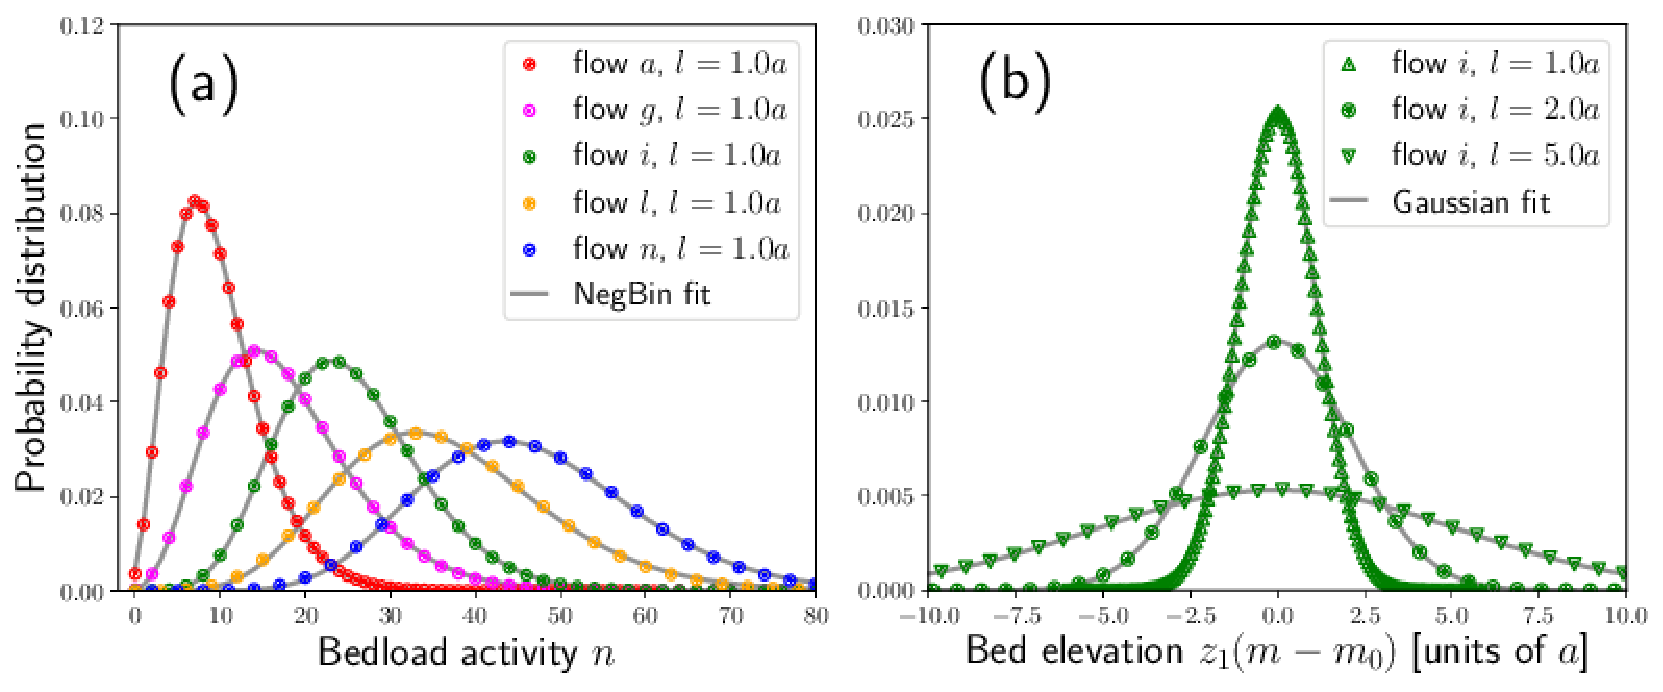
\includegraphics[width=\linewidth,keepaspectratio]{./figures/montage2.pdf}
	\caption{Marginal distributions for $n$ and $m$ for a small subset of simulations. Some points have been omitted for clarity.}
	\label{fig:pdfs}
\end{figure}

From the marginal distributions, we calculate means and variances of bedload activity and elevation ($m$).
The mean bed elevation is just the initial condition $m_0$. $m$ fluctuates around this value because it sets the equilibrium position of the elevation-related feedbacks in (\ref{eq:ele}).
The variance of $m$ appears given by $z_1^2 \text{var}(m) = l^2$, as indicated in figure \ref{fig:var}.
$l$ is a measure of bed elevation fluctuations.
The moments of $n$ are more difficult to understand.
Without dwelling on the issue, the moments of $n$ shift with the ratio $l/z_1$, somehow resulting from feedback between bed elevation changes and bedload transport.

\begin{wrapfigure}{r}{0.5\textwidth}
	\centering
	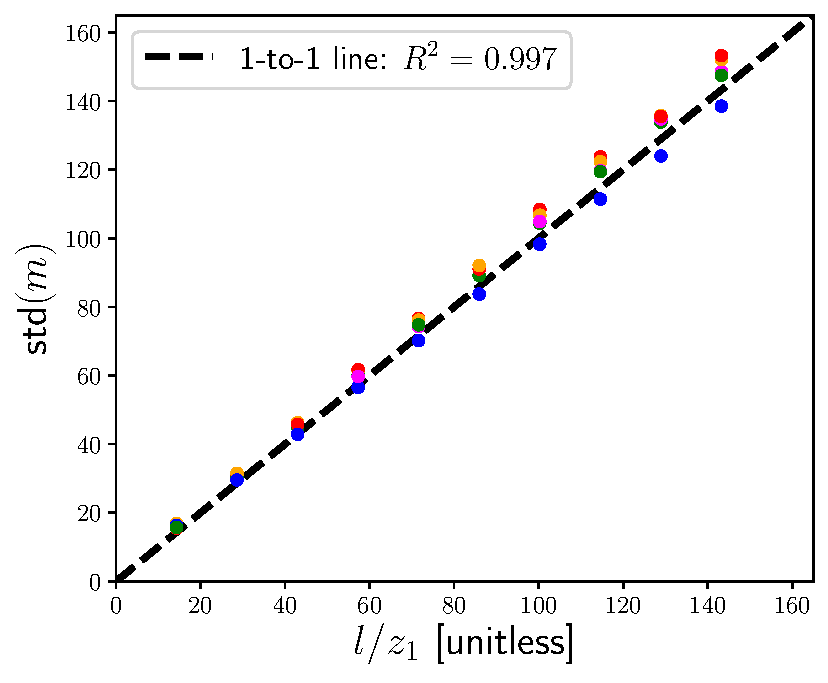
\includegraphics[width=0.5\textwidth,keepaspectratio]{./figures/variance.pdf}
	\caption{Data from all simulations is plotted to show that $l$ controls the standard deviation of bed elevations: $l^2 = z_1^2\text{var}(m).$ We might interpret $l$ as the depth of the active layer \citep[e.g.][]{Church2017}.}
	\label{fig:var}
\end{wrapfigure}

Now we describe the analysis of bedload resting times from time-series of $m$.
Following \citet{Voepel2013} and \citet{Martin2014}, we concentrate on a particular bed elevation $m_\ast$, and find all time intervals separating deposition events at $m=m_\ast$ from erosion events at $m=m_\ast+1$.
Binning these return times to $m_\ast$ and counting the occurrences in each bin (using logarithmically spaced bins for presentation purposes), we obtain a non-exceedance distribution of return times $t_r$ held conditional to the elevation $m_\ast$: $P(T>t_r|m_\ast)$.
Using the marginal probability distribution of bed elevations, we derive the unconditional non-exceedance distribution of resting times as a sum over all elevations \citep{Yang1971, Nakagawa1980, Voepel2013, Martin2014}:
\be P(T>t_r) = \sum_{m'} P(m') P(T>t_r|m') .\ee
Some of these results are displayed in figure \ref{fig:cdfs}..
Comparing panels (a) and (c) shows that the resting time distributions depend on flow condition and the standard deviation of bed elevation ($l$) in different ways.
However, as shown in panels (b) and (d), a characteristic timescale $T_0$ can collapse the tails of the distributions regardless.
\begin{figure}[t!]
	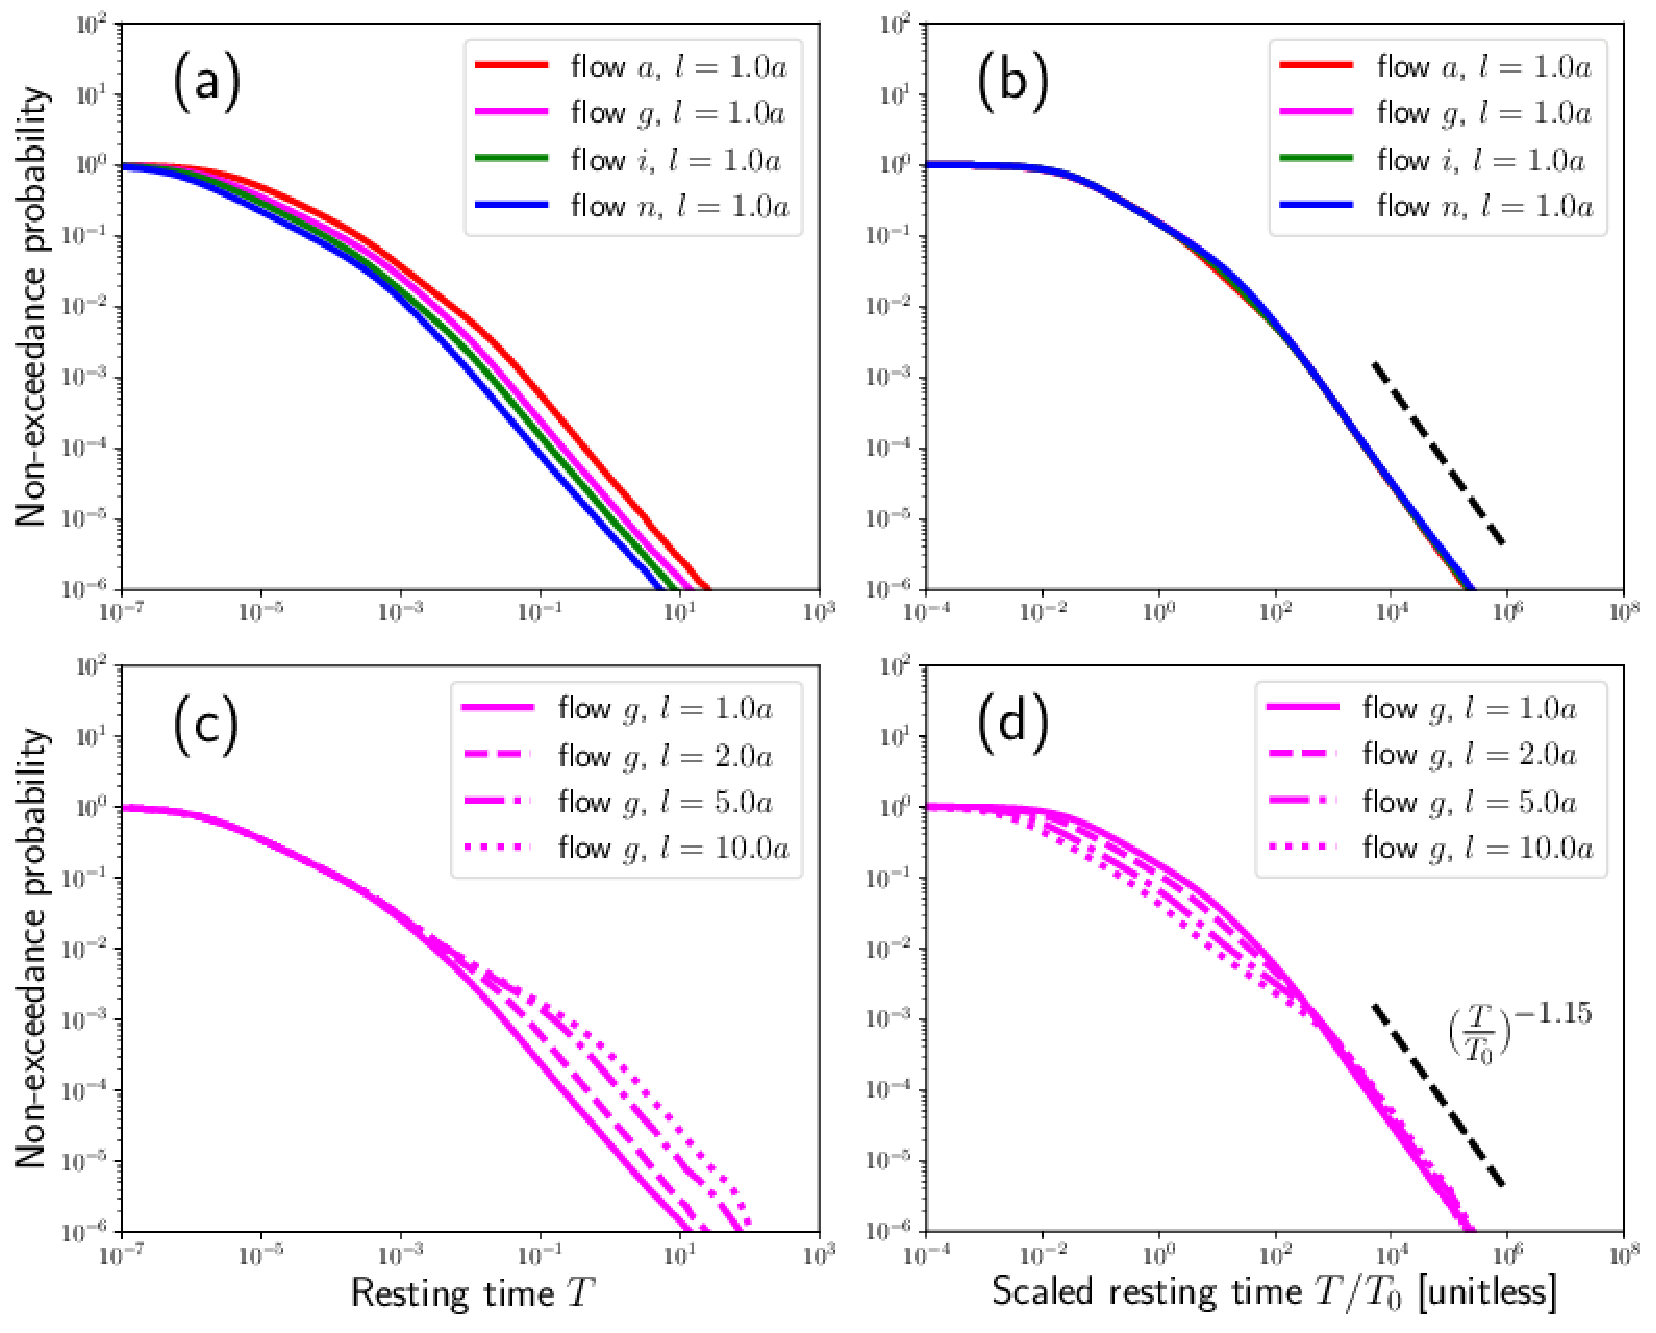
\includegraphics[width=\linewidth,keepaspectratio]{./figures/montage1.pdf}
	\caption{Resting time statistics vary in different ways with flow conditions and the variance of bed elevations. Panel (a) represents differing flow conditions at a fixed $l$ value, while panel (c) is fixed flow conditions at a variable $l$ value. When scaled by $T_0$ (\ref{eq:time}), both of types of difference collapse away in the tails of the distributions, as shown in panels (b) and (d). Finally, in panel (d), the black dotted line indicates a power law decay with tail parameter $\alpha=1.15$ .}
	\label{fig:cdfs}
\end{figure}

Heuristically, we can obtain $T_0$ by thinking of the bed as having a characteristic drift velocity obtained from the mean erosion rate and a certain length scale.
Formally, the mean erosion rate is $E = \sum_{n,m}R_E(n,m)P(n,m)$.
This is the number of grains leaving the bed per unit time.
If bedload transport is in equilibrium, the deposition rate $D$ satisfies $E=D$.
Since the removal of a single grain changes the bed elevation by $z_1$, 
the bed elevations change with a characteristic velocity $z_1 E$.
Since the characteristic deviation of elevation is $l$, the time required for the bed to shift through a characteristic deviation is
\be T_0 = \frac{l}{z_1 E}.\label{eq:time}\ee
This is the timescale collapsing the distributions in figure \ref{fig:cdfs}.
Apparently, for return times roughly satisfying $T/T_0 > 10^3$, all resting time non-exceedance distributions decay as a heavy-tailed power law with parameter $\alpha \approx 1.15$.

\section{Discussion}

Now we summarize our key findings and discuss their scope and implications.
First, we have generalized the stochastic bedload theory of \citet{Ancey2008} to provide a joint description of bed elevations and transport.


\begin{enumerate}
	\item You generalized the stochastic bedload theory of ancey to provide joint description of bedload transport and bed elevation changes, including fluctuations and feedbacks. \citet{Ancey2008} was a single cell model of bedload transport which was generalized in \citet{Ancey2014a} to an $N$ cell model. This facilitated the study of spatial correlations in transport in \citet{Heyman2014}. Could the single cell model developed here be a first step toward a stochastic framework from which to study morphology? 
	Maybe, but closure would be a nightmare \citep[e.g.][]{Heyman2016}.
	
	
	\item Now we draw connections to earlier work. The master equation (\ref{eq:8}) has limits of $l\rightarrow 0$ and $l \rightarrow \infty$ which generate the theories of \citet{Martin2014} and \citet{Ancey2008} as limit cases.
	\item We predict the expected form of the resting time distribution which wouldl be expected in narrowly graded sediment under equilibrium sediment transport. Of course, it's unclear to what extent this corresponds to a natural stream. At the very least, it's apparently true that flood cycles can sometimes be treated as equilibrium even though they're conceptually not \citep[e.g.][]{Phillips2013}.
	\item Our resting time distributions collapse to an identical tail for $T/T_0>10^3$ where $T_0 = l/(z_1 E)$ is a characteristic timescale of bed elevation change.
	This implies anomalous superdiffusion of bedload tracers. Can describe what this entails.. infinite slowdown of tracers and so on.
	\item Finally, we corroborate the study of \citet{Martin2014}.
	He gets similar results. However, his theory did not address sediment transport, and his scaling was not complete. Specifically, because the depth of the active layer shifts with discharge, and Martin was only scaling with the factor $E$, his experiments show a systematic drift in the tail of the resting time distribtuions that would not collapse away. That's because he didn't involve $l$. 
	\item Deriving a bed elevation theory from the basis in sediment transport implies equations which do not reproduce or relate to \citet{Voepel2013}. The concepts in this theory are useful, but the treatment of bed elevations as a bounded random walk without persistence are incorrect. The OU process of \citet{Martin2014} is more appropriate, especially if it's ammended to include $l$. 
	\item four implications: (1) joint stochastic theory, (2) heavy-tailed resting times, prototypical, $\alpha = 1.15$, (3) anomalous superdiffusion of bedload tracers is expected if burial occurs, (4) however, there is still no proof that burial is the mechanism of burial.. discuss \citet{Bradley2017} suggestion of multiple return processes occurring simultaneously in a channel, highlight the possibility that some of them are even heavier-tailed than burial, which means when they act they obscure the burial signature (i.e. the 1.15 tail of me and Martin.)
\end{enumerate}




Of course, a great deal of effort has been devoted to modeling the coupling between sediment transport and morphology \citep[e.g.][]{Pelosi2014}.
However, to our knowledge, the simple population dynamics theory of bed elevation changes and transport we've presented here might be the first example of a morphodynamics theory 


ay be the first example of what might be called a Lagrangian theory of morphodynamics.
That is, a means to predict morphodynamics -- in this case just simple bed evolution, from modeling the motion characteristics of individual grains.
In closure to this first point, we note the \citet{Ancey2008} model of bedload transport based on a single cell was subsequently extended to an array of adjacent cells \citep{Ancey2014a}, generated a framework which \citet{Heyman2014} used to study spatial correlations in bedload transport.





\begin{comment}
\begin{enumerate}
	\item generalized ancey2008 to obtain a joint description of elevation and bedload
	\item relation to other work. show limits from the master equation to ancey and martin/voepel/tsujimoto
	\item how do multiple return time signals mix? Is burial preserved in the signal?
	\item implications for tracer studies -- this is a prototypical model of burial
	\item if nature is similar, diffusion is anomalous and tails are alpha =1.1
	\item key implication: describe other return processes. if these mix and don't
	pollute the signal, then this theory applies to tracers in the field 
\end{enumerate}
\end{comment}

\section{Conclusion}

Conclude by wrapping discussion with introduction and implications especially. 1 paragraph 




\begin{comment}


%%%%%%%%%%%%%%%%%%%%%%%%%%%%%%%%%%%%%%%%%%%%%%%%%%%%%%%%%%%%%%%%%%%%%%%%%%%%%%

One simulated realization of our joint stochastic process for bed elevations and bedload transport is depicted in figure \ref{fig:pdfs} (a). 
These realizations determine the joint statistics of $n$ and $m$. 
The bedload transport statistics are depicted for a subset of all simulation conditions in figure \ref{fig:pdfs} (b). 
The \citet{Ancey2008} theory predicts negative binomial distributions for the number of moving grains within the control volume, and the mathematical form of these distributions is apparently not changed by our extension to account for feedbacks between bed elevation changes and entrainment and deposition probabilities.
We obtain an excellent negative binomial fit to the marginal probability distribution of $n$, $P(n) = \sum_m P(n,m,t)$, for all 40 of our simulation results.
However, activity statistics, including the mean activity and its variance, are definitely shifted by the inclusion of differential mobility with bed elevation changes.
Bed elevation changes appear to buffer the magnitude of bedload fluctuations by up to 30 percent, which is an expected effect of the model, since a rapid increase in the bedload rate induced by a series of many entrainments will lower the bed elevation and increase the probability of deposition, buffering the magnitude of the bedload rate increase.

\begin{figure}[t!]
  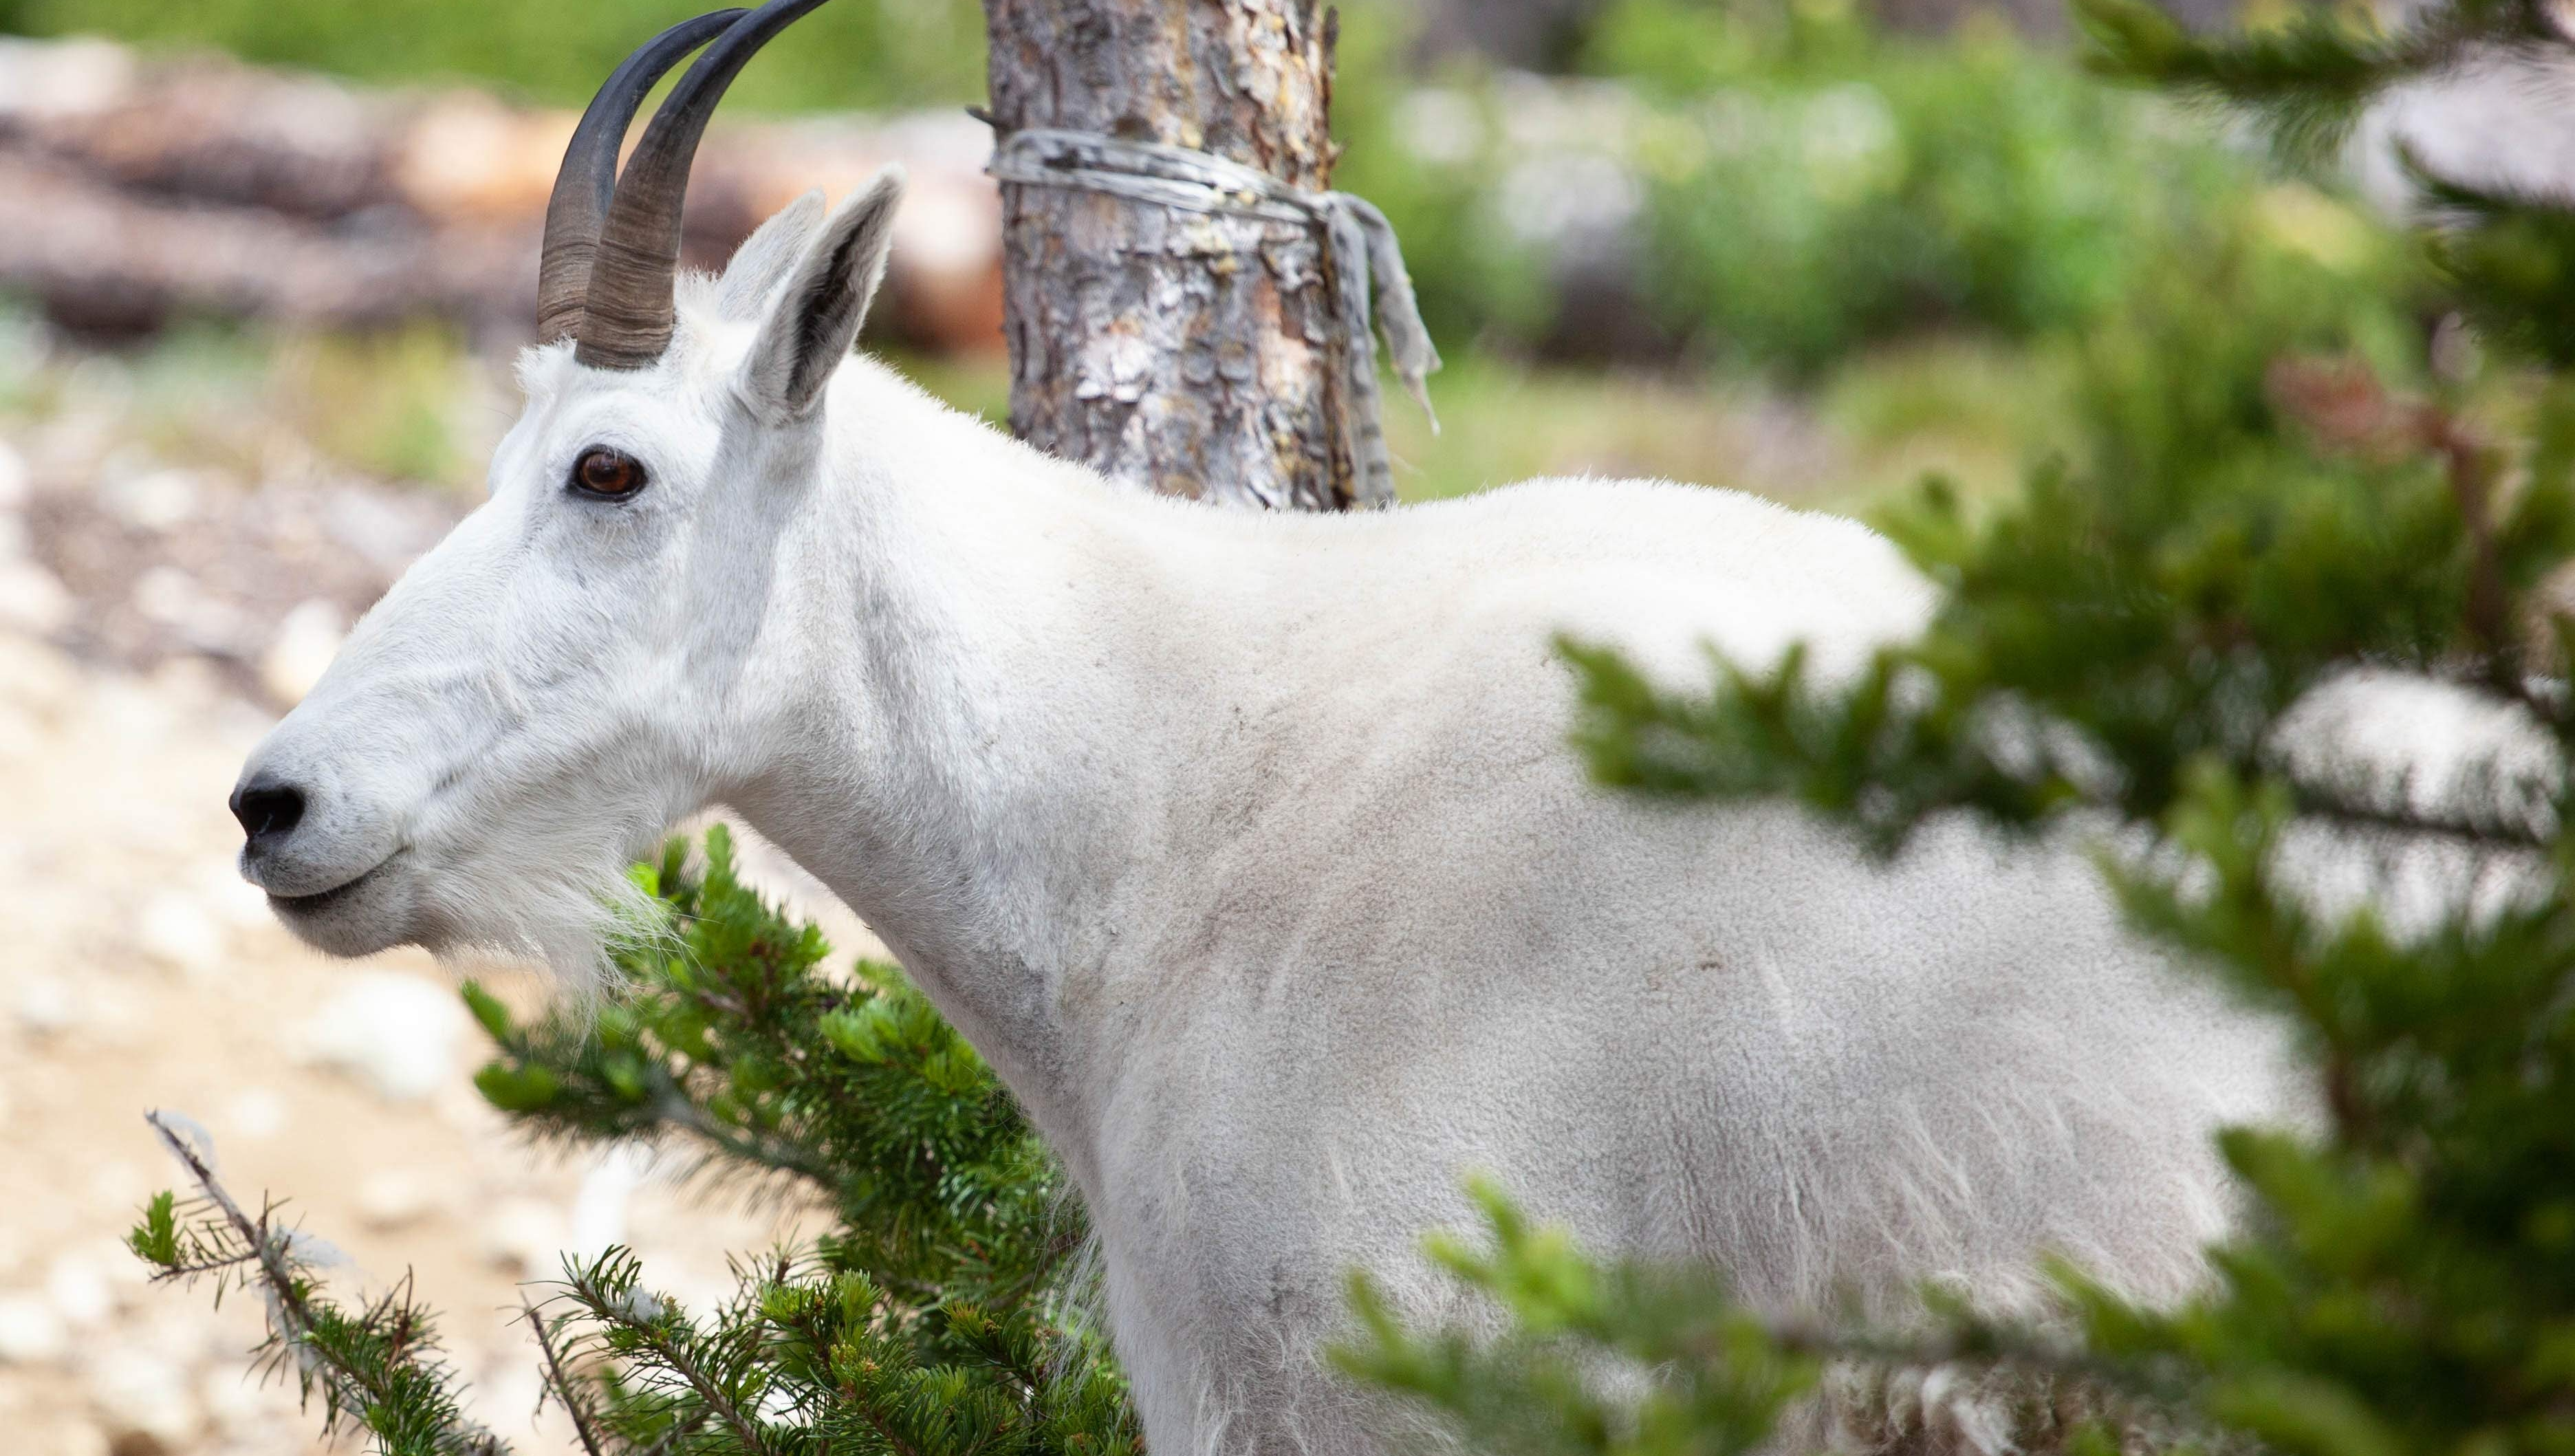
\includegraphics[width=\linewidth,keepaspectratio]{rectdummy}
  \caption{Figure (a) depicts timeseries of particle activity and bed elevation over a $20$ minute interval. Figures (b) and (c) display probability distribution functions of bed elevation (equation \ref{eq:ele}) and particle activity for a subset of the simulations. Colors represent flow conditions, while differing line styles represent different values of the differential mobility parameter $l$.}
\vspace{-1.0cm}
  \label{fig:pdfs}
\end{figure}

Our bed elevation timeseries exhibit longer temporal correlations than related bedload activity series, evident in figure \ref{fig:pdfs} (a). 
All 40 of our simulations develop clean unimodal distributions of bed elevations which are fit by Gaussian distributions with excellent correlation, and a subset of these marginal bed elevation pdfs with their Gaussian fits are displayed in figure \ref{fig:pdfs} (c). 
The mean number of particles resting on the bed is $m_0$, corresponding to a relative elevation $z(m_0)=0$. 
The variance of bed elevations is controlled by the differential mobility parameter $l$. 
Apparently, the simulations support the conclusion that $var(m) = (l/z_1)^2$. 
This conclusion is evident in figure \ref{fig:var}, with generally excellent correpsondence between this relationship and the simulation points, with some scatter we attribute to the finite duration of our simulations.

To compute the resting time distribution; at each elevation $m$, we extract the set of all departure times from this elevation, or times at which the bed was at this elevation and a deposition occurred; then we extract the set of all return times to this elevation, or times at which the bed was one increment above this elevation ($m+1$) and an entrainment occurred.
Taking differences between these two time-series returns the set of all return times from above marginal to the elevation $m$, which we binned across a $0.5$s interval to compute the cumulative probabilities of return times at each elevation m, $P(T_r>t|m)$.
Following earlier investigators, we computed the unconditional or over-all rest time distribution as the convolution of these conditional distributions over all bed elevations \citep[e.g.][]{Yang1971, Voepel2013}:
\be P(T_r>t) = \sum_m P(m) P(T_r > t| m), \ee
where $P(m)$ is the pdf of bed elevation like those depicted in figure \ref{fig:pdfs} (b) and the sum is over all bed elevations attained during the simulation. 

\begin{wrapfigure}{r}{0.5\textwidth}
\centering
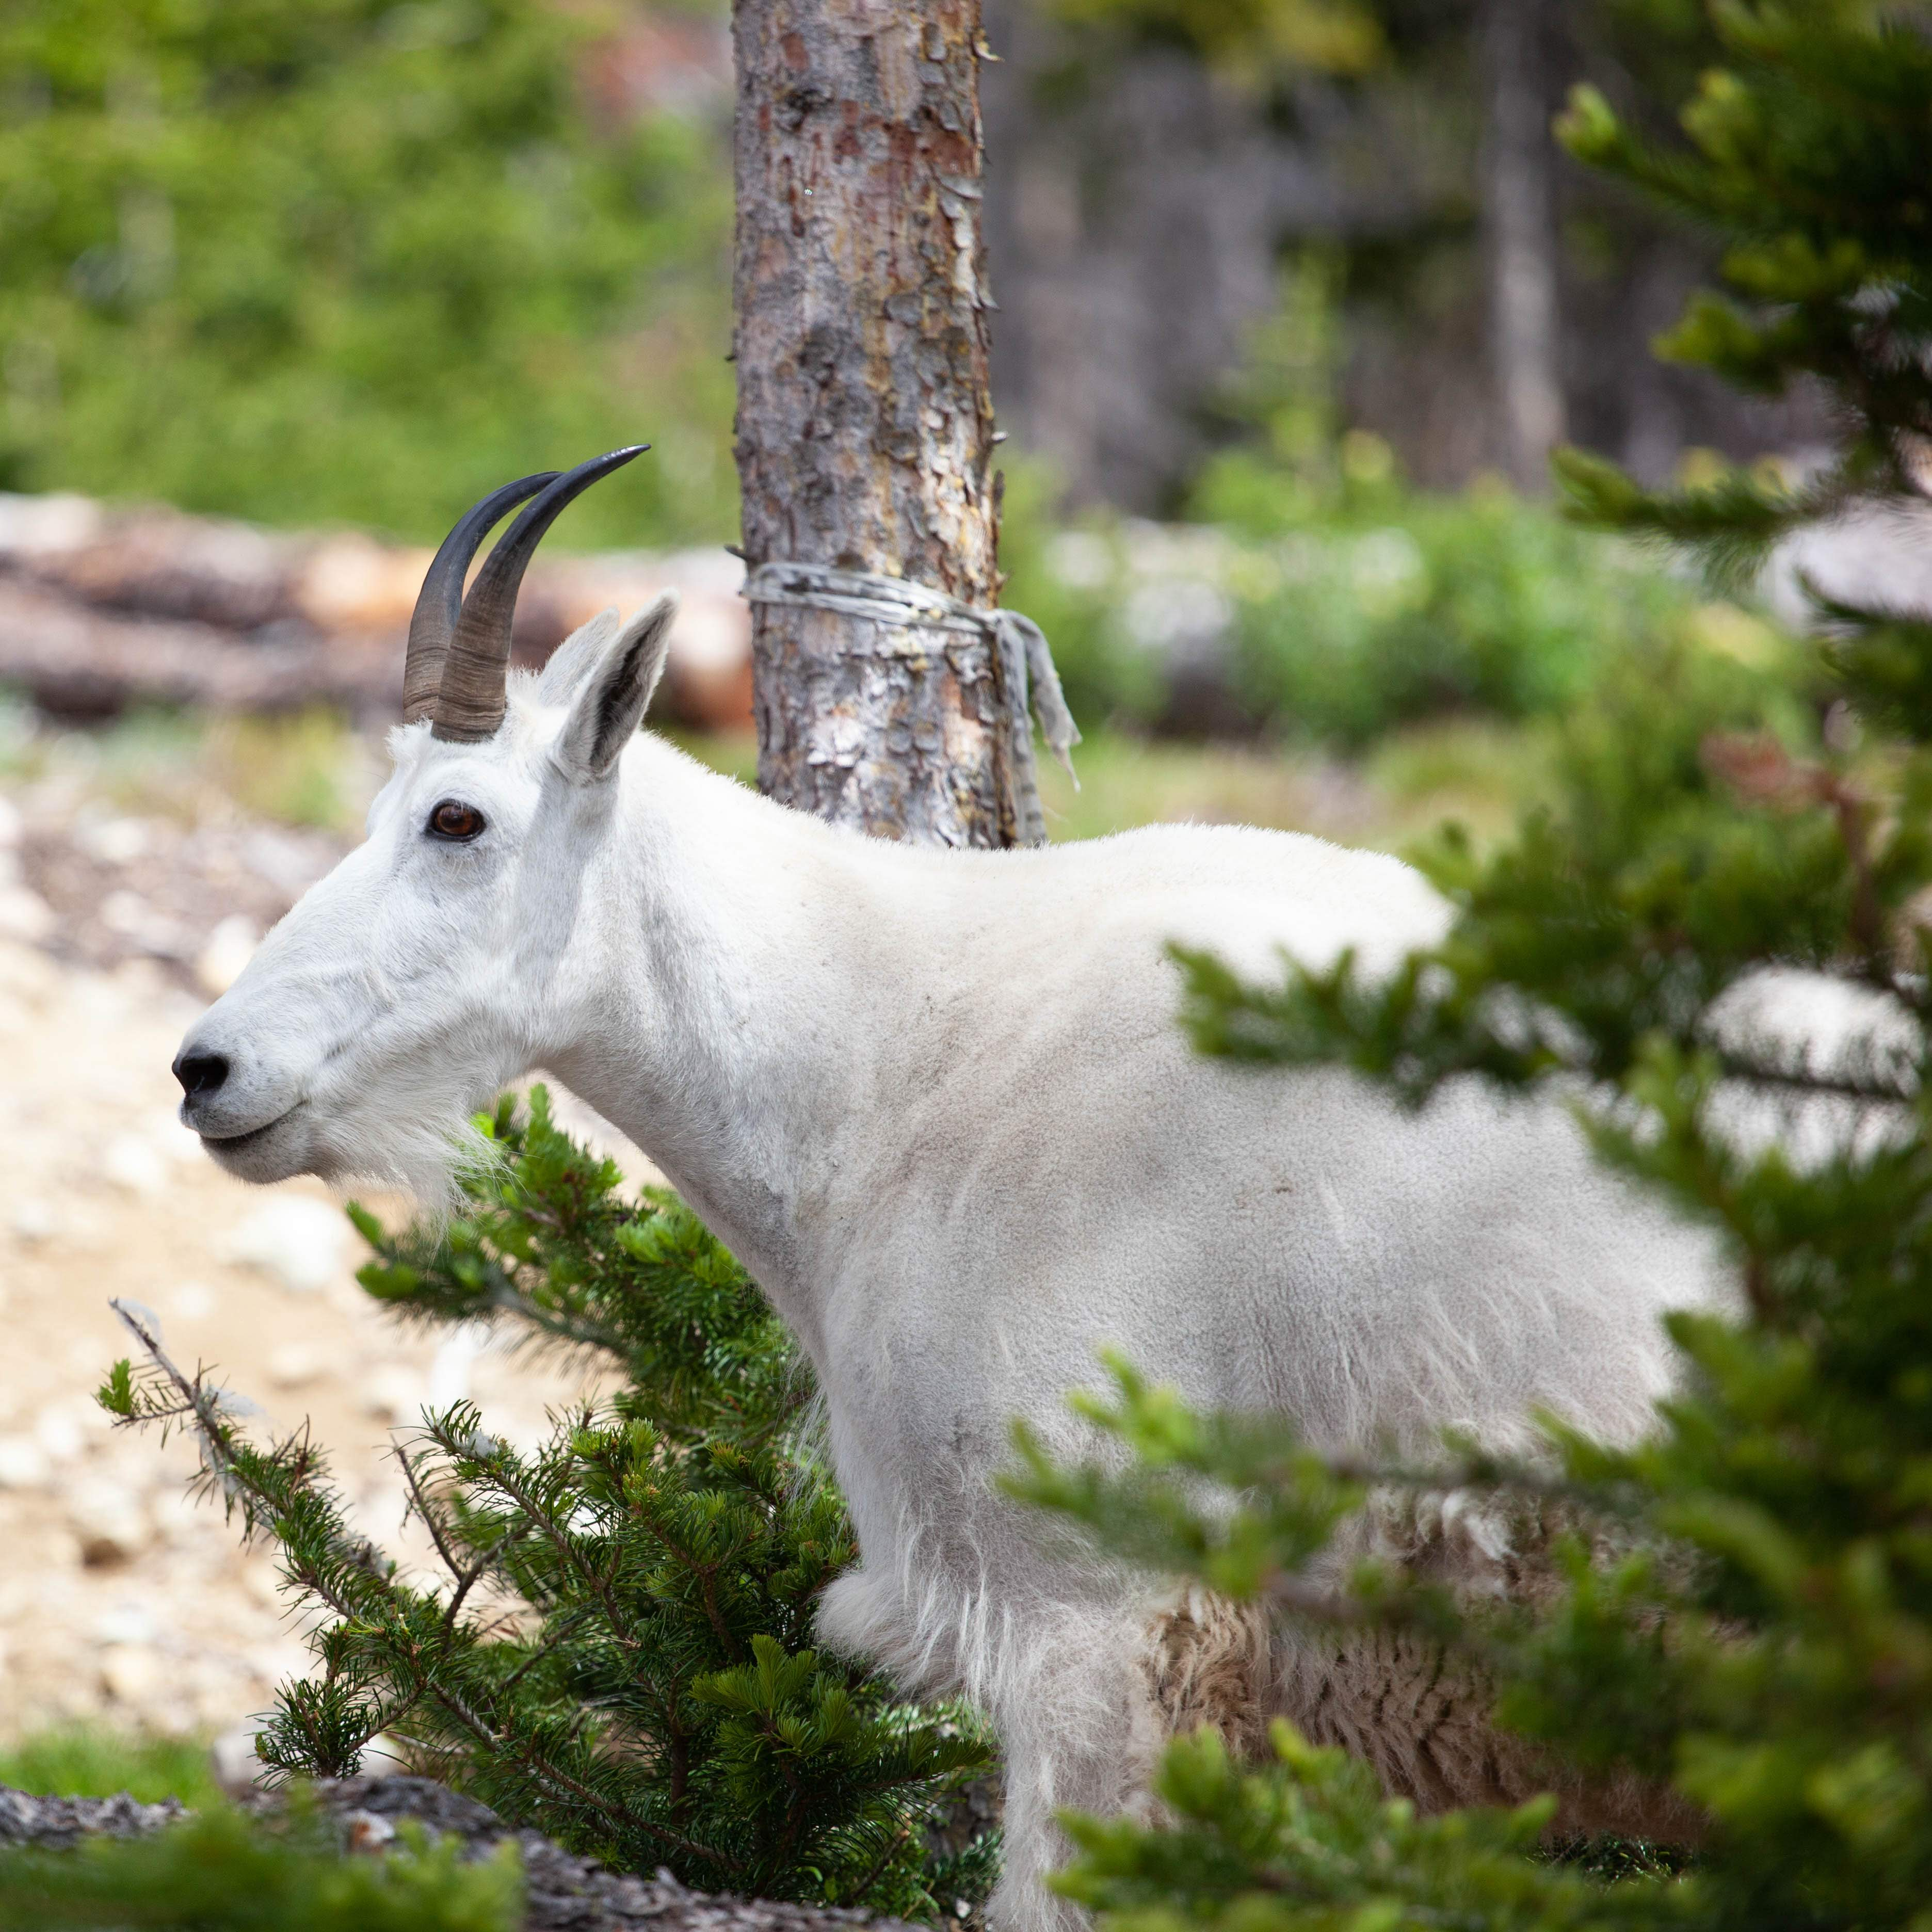
\includegraphics[width=0.5\textwidth,keepaspectratio]{squaredummy}
\caption{The standard deviation of bed elevation scales one-to-one with the differential mobility parameter $(l/z_1)$, indicating the ratio $l/z_1$ controls the magnitude of bed elevation fluctuations. }
\label{fig:var}
\end{wrapfigure}

This analysis derives unconditional exceedance probabilities of resting times with heavy power-law tails. 
A subset of all of our simulation results are depicted in figure \ref{fig:collapse} (a)-(d). 
Apparently, for suitably long times, the tail parameter $\alpha$ of these resting time distributions is independent of flow conditions or the differential mobility parameter $l$. 
However, the timescale at which particle resting transitions from exponential to power-law scaling shifts with flow conditions and $l$. 
\citet{Martin2014} obtained an approximate collapse at the tails of their experimental resting time distributions using the reciprocal of the rate of entrainment or deposition events occurring. They denoted this rate by $a$, so that their timescale was $1/a$.
Scaling the resting times by $1/a$ provides an incomplete collapse of the tails of our simulated resting time distributions, which may describe the incomplete collapse of the experimental data of \citet{Martin2014}.  
It collapses the tails across flow conditions when $l$ (the standard deviation of bed elevation) is fixed, i.e., it leads to the collapse seen between figures \ref{fig:collapse} (a) and \ref{fig:collapse} (b), but if $l$ (which is the standard deviation of bed elevation) varies with flow, then the power-law scaling of resting times is no longer controlled by $1/a$ alone. 
Instead, we must include a factor representing the differential entrainment and deposition characteristics of grains as the bed elevation changes. 
The timescale which provides universal collapse of the power-law tails of all our simulations is $T_0 = l/(z_1E),$ where $E$ is the entrainment rate.

\begin{figure}[t!] % t for top and ! for force it 
  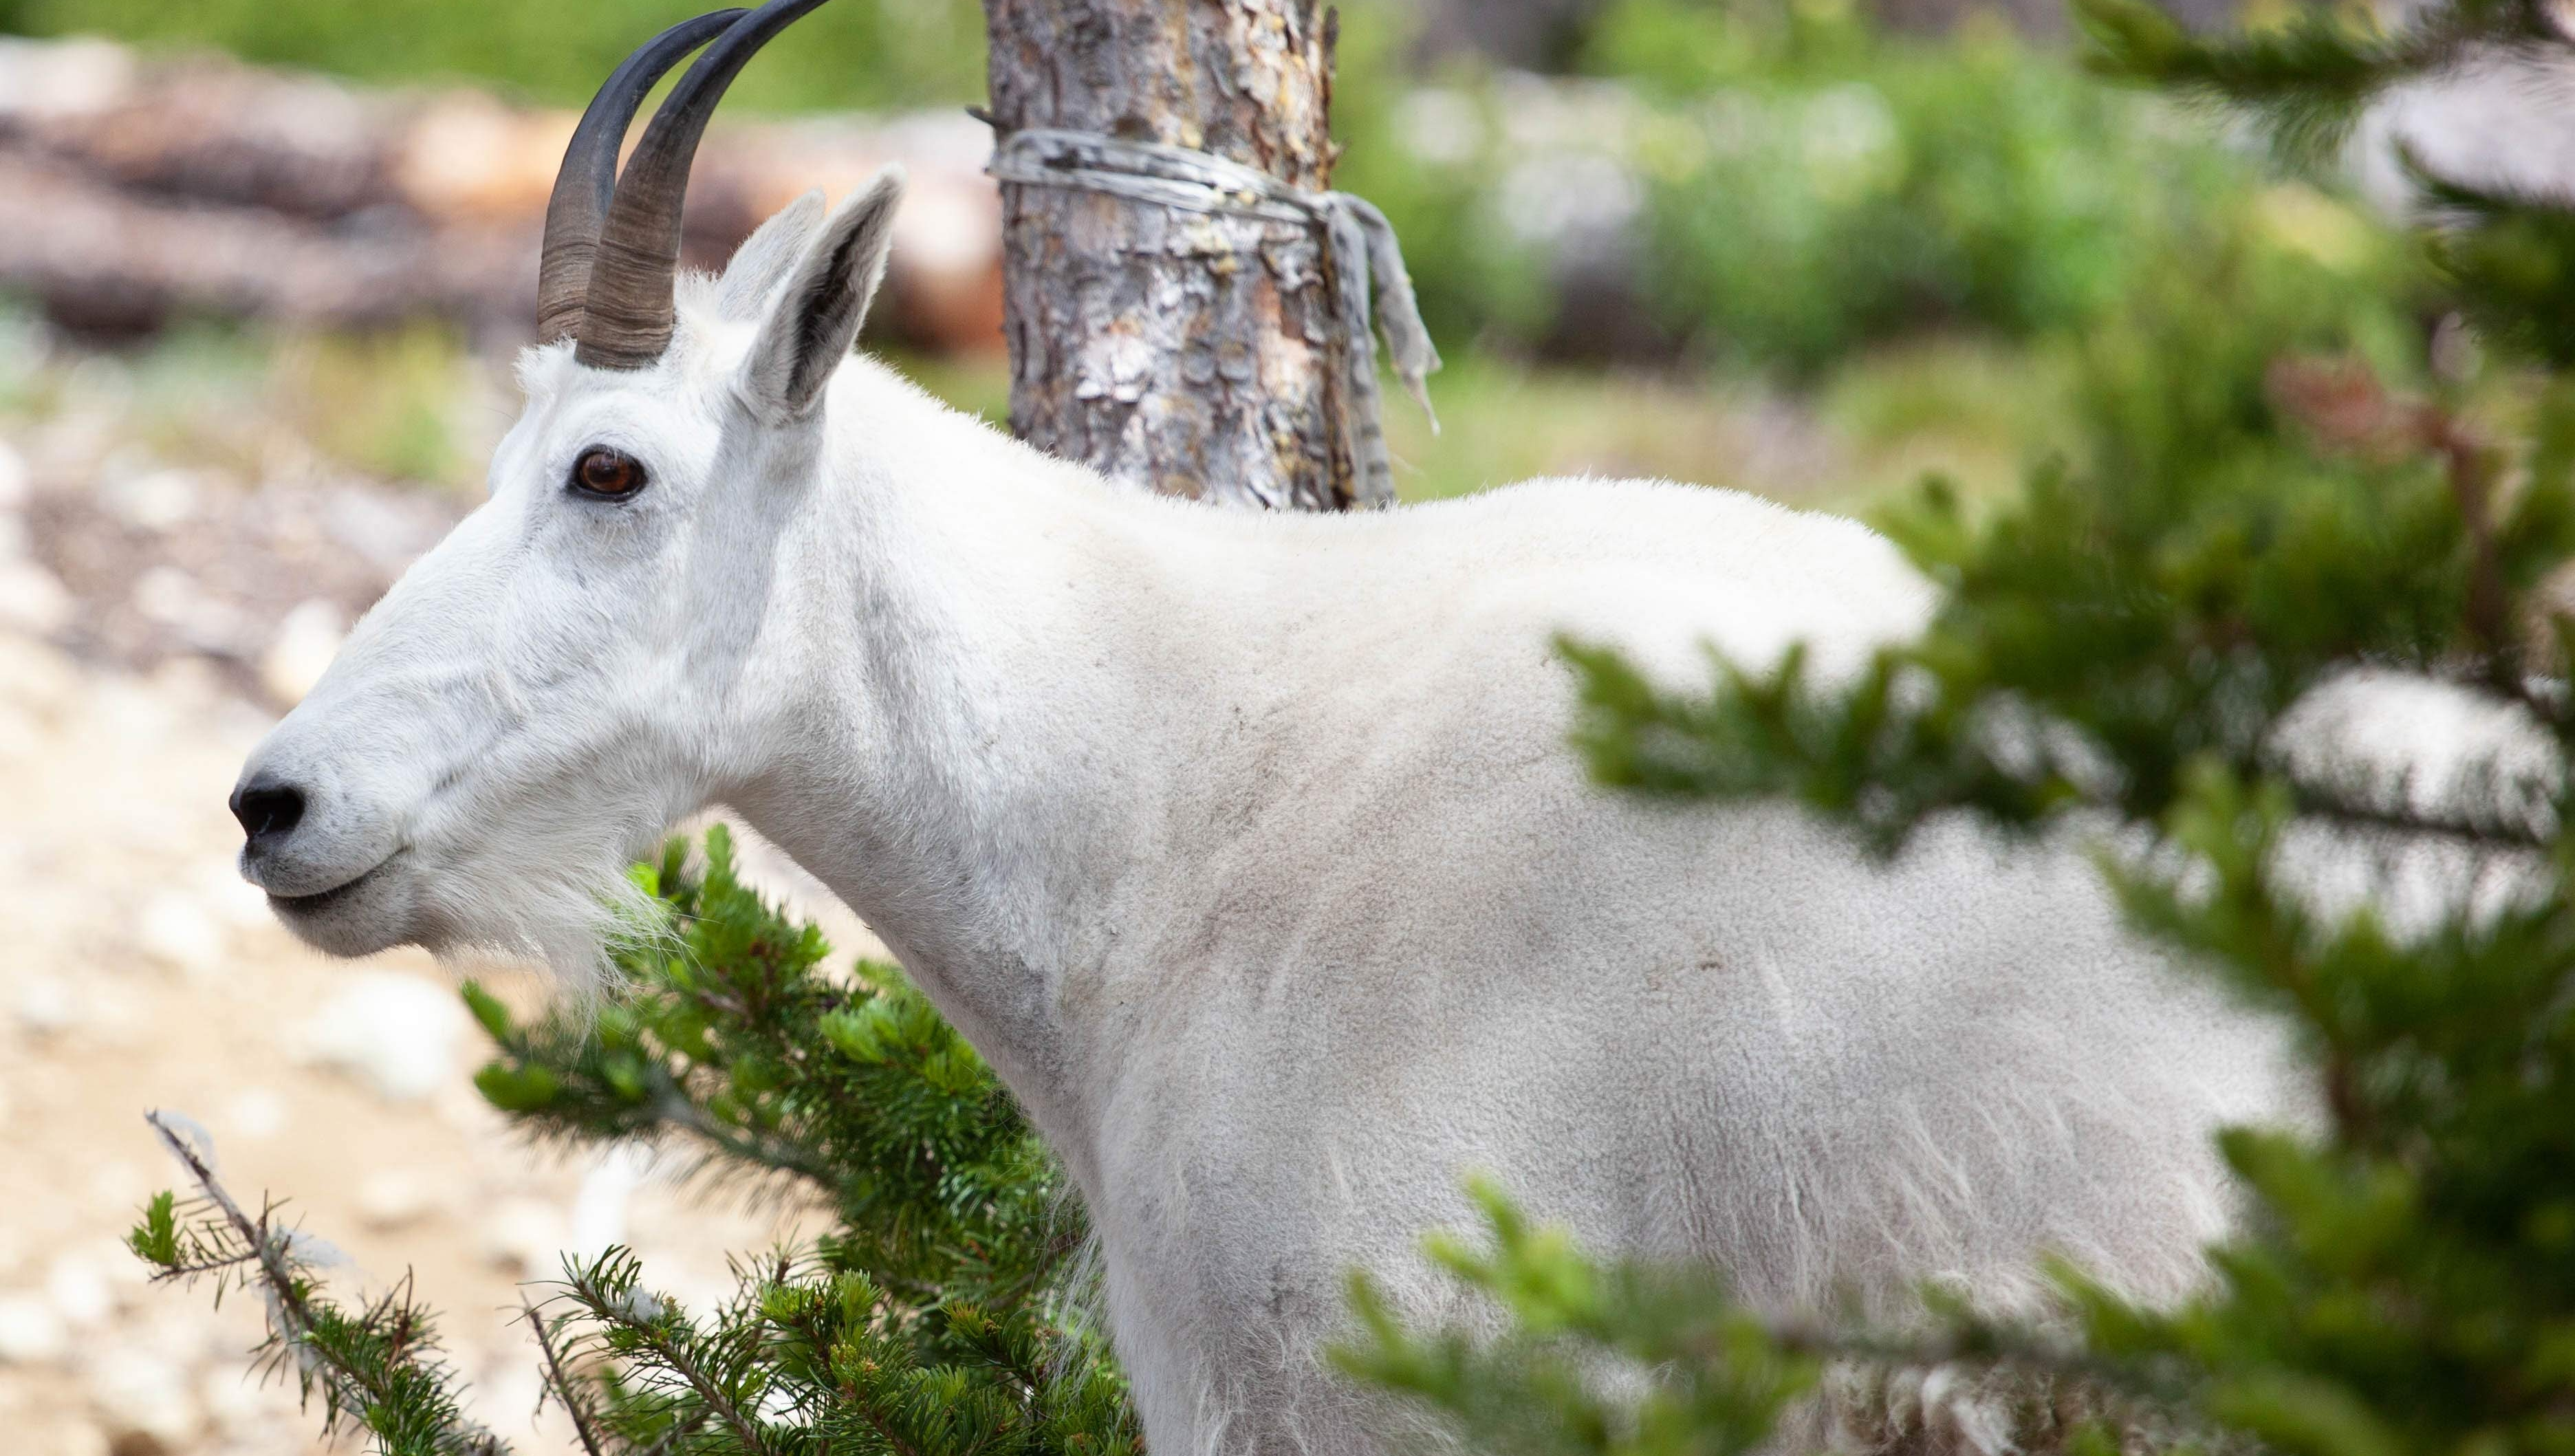
\includegraphics[width=\linewidth,keepaspectratio]{rectdummy}
  \caption{This figure summarizes the resting time exceedance distributions for a subset of all simulations. Part (a) displays resting time distributions for a range of flow conditions at fixed $l$, while part (b) displays the collapse obtained by scaling $T_r$ by $T_0$. The collapse between (a) and (b) is analogous to \citet{Martin2014}, and it is induced by the factor of $1/E$ within $T_0$. Parts (c) and (d) display a similar collapse for a fixed flow condition at variable $l$. In this case, collapse is driven by the factor of $z_1/l$ within $T_0$, and this influence of differential mobility in resting statistics has not to our knowledge been noticed up to now.}
\vspace{-1.0cm}
  \label{fig:collapse}
\end{figure}

We can understand $T_0$ with a physical argument.
According to figure \ref{fig:var}, the typical length scale of bed elevation fluctuations is $l$, and as mentioned the length scale $z_1$ is the magnitude of bed elevation change enacted by the entrainment or deposition of a single particle.  
In equilibrium bedload transport, \citet{Einstein1950} tells us the condition $E=D$ holds: this is a statement of mass conservation. 
Since $E$ represents the mean number of particles removed from the bed in a unit of time, the product $E z_1$ can be interpreted as a representative velocity scale of bed return. 
It is the distance the bed lowers with the removal of a single particle divided by the mean time required to remove it.
Hence we extract our timescale as a key distance scale over a key velocity scale: $T_0 = l/(z_1 E).$ 
Scaling the resting time as $T_r/T_0$ exhibits a consistent power-law tail across all of our simulation results. 

\section{Discussion}

Our theory of bed elevations derives results similar to \citet{Martin2014} using bedload transport as a starting point, and it also provides a statistical characterization of bedload transport.
Our assumptions derive a heavy-tailed power-law distribution of resting times with a tail parameter $\alpha \approx 1$ which displays differences across flow conditions which partially collapse upon scaling by an activity timescale.

However, in extension of the \citet{Martin2014} theory, our model reveals another timescale which fully collapses the power-law tails of the resting time distributions, suggesting a universal power-law should characterize the asymptotic resting times of sediment undergoing burial if the assumptions of our model are correct.
This timescale includes an additional factor characterizing the dependence of entrainment and deposition probabilities on changes in local bed elevations.
We hypothesize this new factor may explain some of the differences between field \citep[e.g.][]{Olinde2015} and laboratory \citep[e.g.][]{Martin2014} observations of resting time distributions, providing additional information to determine whether burial is the dominant mechanism of the heavy-tailed sediment resting times observed in natural channels.


Pierce
The model describes why Martin et al (2014) obtained incomplete collapse between their resting time distributions. They didn't include the $(z_1/l)^2$ type factor in their scaling time-scale
It is a first joint stochastic description of bed elevations and bedload transport, mixing martin 2014 and ancey 2008. 
It provides a mechanism for heavy-tailed resting times and implies super-diffusion of bedload and a virtual velocity of sediment which decreases toward zero with time. 
 what else? help



Hassan
1.      Discuss what is special in the model and how it works. (most of point number 2)

2.      Your point number 1

3.      The last pargraph from the introduction

4.      Your point number 3 with implications (What this means for the study of bedload (and channel morphology in streams). The implications should be short.


\section{Conclusion}
 
Bedload diffusion is anomalous because of heavy-tailed sediment resting times \citep{Bradley2017}.
Several theories have shown that heavy-tailed resting times should result from sediment burial \citep{Voepel2013, Martin2014}, and a few experiments have resolved heavy-tailed resting times within natural channels \citep{Olinde2015, Bradley2017}, but these experiments do not support a consensus on the power-law decay, truncation properties, or scaling behavior of the resting time distribution.
Bedload transport and bed elevations vary randomly, so we have pursued a joint stochastic model of these quantities based on a juncture of earlier works \citep{Ancey2008, Martin2014}.
Following the classic literature to interpret burial times as the return time from above in the bed elevation time series \citep{Yang1971, Nakagawa1980}, and including the effect of mobility variation with local bed elevation changes \citep{Sawai1987, Wong2007, Martin2014}, we obtained at a few key conclusions regarding the resting time of sediment undergoing burial.
 
First, particle activities lie on negative binomial distributions, meaning they exhibit relatively wide bedload transport fluctuations. 
This result is essential unchanged from the \citet{Ancey2008} theory, except the moments of the particle activity distribution do shift as a result of bed elevation changes. 
In this work we have chosen to neglect this topic to support a more careful discussion of resting times, but this observation of a negative feedback between bedload fluctuations and bed elevation changes is worth a more careful analysis. 
Second, bed elevations lie on Gaussian distributions, reflecting symmetrical variations in bed elevations, and thin tails which suppress but do not prohibit extreme bed elevation variations.  
Third, and most importantly, the resting time of stationary sediment undergoing burial lies on a heavy-tailed distribution which decays as a power-law with tail parameter $\alpha \approx 1.0$. Our resting time distributions are truncated at a timescale related to the period of observation, and we uncover universal scaling in the power-law decay of these distributions by the timescale $T_0 = l/(z_1E)$.

The timescale $T_0$ is derived from a physical argument: it is the ratio of the representative length scale of bed elevation variations $l$ with a velocity scale of bed elevation changes $z_1 E$. 
Conceptually, $1/E$ is equivalent to the timescale $1/a$ used by \citet{Martin2014} to attain a partial collapse of their resting time distributions across various flow conditions.
Actually, the rate $a$ of entrainment or deposition occurring is $a \approx E+D$, and in equilibrium bedload transport we have $E\approx D$ \citep{Einstein1950}, so $E = a/2$. 
To fully collapse our simulated resting time distributions, the timescale $1/E$ is not sufficient: it collapses across variations in flow but it does not collapse the power-law tails across the concordant variations in the magnitude of bed elevation fluctuations ($l$).
This observation suggests the incomplete collapse of the power-law resting time tails of the \citet{Martin2014} flume experiments, and the appreciable variability of the \citet{Olinde2015} field experiments might be attributed to the differential mobility of bed particles with bed elevation changes, which our model encodes in the ratio $l/z_1$.

In conclusion, we highlight that sediment burial under a region of bed under-going active bedload transport, as we have modeled here, is probably only one mechanism from which natural rivers might express the heavy-tailed sediment burial time distributions which have been observed in tracer experiments \citep{Voepel2013, Olinde2015,Bradley2017}.
The resting time distributions we have simulated, although they have satisfying correspondence with the laboratory experiments of \citet{Martin2014}, where heavy-tailed resting times are verifiably controlled by burial, have limited explanatory power over the excellent field data of \citet{Bradley2017}, which were obtained from a 9 year series of tracer observations.
In natural channels, other mechanisms may induce heavy-tailed resting times of sediment: \citet{Bradley2017} suggested we might look to other stochastic return processes within fluvial channels, such as the return of water levels to tracer particles stranded high on a bar, to gain understanding of sediment resting times.
Similarly, \citet{Malmon2005} suggested sediment residence within floodplains is controlled by the timescales of river channel migration, meaning the resting times of sediment really link to a host of processes from the compounded timescales of individual granular movements, like we have modeled, up to intermediate timescales related to the intermittency of floods, as suggested by \citet{Bradley2017}, all the way up to morphological timescales such as those characterizing channel migration.

Probably, for considerations of contaminant evacuation from gravel bed rivers on typical timescales of ecological relevance (decadal, centennial), a predictive understanding of sediment resting will require the former two processes: sediment burial and water level return. 
In this work, we hope we have created new understanding of the former, uncovering some universal scaling properties.  
The latter topic, which was suggested by Bradley but has not yet been studied, deserves immediate research attention.
According to our model, sediment burial alone is enough to induce fluvial sediment resting time distributions with heavy tails sufficient to drive an arbitrary slowdown of tracer particles or solid contaminants as their period of residence in the channel is increased, and we can state confidently that under idealized conditions when the assumptions of \citet{Einstein1950} are valid, this heavy-tail will decline approximately as $P(T_r) \propto (T_r/T_0)^{-1}$, but we have no idea how these conclusions would be modified by multiple return processes acting in concert, although we hypothesize this could explain the relatively slower decays seen in field data, for example the values of $0.31<\alpha<0.72$ of the \citet{Olinde2015} experiments.
We hope to see subsequent theories deriving resting times from more general channel return processes acting in coordination, and a proliferation of experiments, so we can pin down a mechanistic theory of anomalous diffusion and fluvial contaminant transport.
\end{comment}
\acknowledgments
The simulation code is available upon request from the first author. We would like to thank Shawn Chartrand and Conor McDowell for helpful discussions. 

\bibliography{biblio}

\end{document}




